\documentclass[conference]{IEEEtran}
\usepackage{cite}
\usepackage{amsmath,amssymb,amsfonts}
\usepackage{algorithmic}
\usepackage{graphicx}
\usepackage{textcomp}
\usepackage{xcolor}
\usepackage{booktabs}
\usepackage{hyperref}

\begin{document}

\title{Analytical, Numerical, Neural, and Hybrid Inverse Kinematics\\
on a Low-Cost 3D-Printed 5-DOF Arm:\\
Why the Bottleneck Is Mechanical, Not Algorithmic}

\author{
\IEEEauthorblockN{Student 002}
\IEEEauthorblockA{\textit{Robotics Laboratory} \\
\textit{University Name}\\
City, Country \\
email@example.com}
}

\maketitle

\begin{abstract}
Inverse kinematics (IK) is usually studied as a purely algorithmic problem, under the implicit assumption that the robot's kinematic parameters are known exactly. This assumption breaks down for the growing class of low-cost, 3D-printed, hobby-grade manipulators, where link lengths and joint offsets deviate from their nominal CAD values by amounts large enough to dominate the error budget. We study this regime on the LeRobot SO-101, a 5-degree-of-freedom (DOF) desktop arm, by implementing and comparing four IK methods: (1) a closed-form analytical solver based on geometric decomposition, (2) a damped least squares (DLS) numerical solver, (3) a multi-layer-perceptron (MLP) neural solver trained on \emph{real} robot data, and (4) a hybrid that warm-starts DLS from the network prediction. In software, the methods span more than two orders of magnitude in accuracy: the analytical solver, fed the nominal (inaccurate) link lengths, fails on all but a handful of targets ($244$~mm mean, $4/50$ success), while the numerical solver reaches $0.9$~mm. Yet when the \emph{same} solutions are executed on the physical arm, all methods collapse onto a common $\sim\!34$~mm error floor. We show through a direct joint-command experiment that this floor is a \emph{mechanical} error---dominated by $\approx\!4.6^{\circ}$ of gravity-induced shoulder sag---and is essentially independent of the IK algorithm. Finally, we demonstrate that a simple joint-space closed loop using only the servos' own encoders reduces the real-robot error from $33.6$~mm to $4.0$~mm ($88\%$ reduction) without any external sensing. Our results reframe the practical IK question for low-cost arms: solver precision beyond the mechanical floor is wasted unless closed-loop compensation is added. Code and the real-robot dataset are released for reproducibility.
\end{abstract}

\begin{IEEEkeywords}
inverse kinematics, robot manipulator, neural networks, damped least squares, hybrid methods, kinematic calibration, closed-loop control
\end{IEEEkeywords}

\section{Introduction}

Inverse kinematics (IK) computes the joint configuration $\mathbf{q}$ that places a manipulator's end-effector at a desired task-space pose \cite{siciliano2016robotics}. It is a cornerstone of task-space control, and decades of work have produced analytical \cite{craig2005introduction}, numerical \cite{buss2004introduction}, and, more recently, learning-based \cite{duka2014neural, bensadoun2022neural} solvers.

Almost all of this work is evaluated either in simulation or on industrial arms whose kinematic parameters are known to sub-millimeter precision after factory calibration. A different and increasingly common situation is the low-cost, open-source, 3D-printed manipulator---exemplified by the LeRobot SO-101 used here---assembled by hand from printed parts and hobby servos. For such arms, the nominal (CAD/URDF) link lengths and joint zero-offsets can be wrong by several millimeters and several degrees. This raises a question that the classical IK literature rarely addresses directly: \emph{when the model itself is inaccurate, does the choice of IK algorithm still matter?}

This paper answers that question empirically. We implement four IK methods of increasing data-dependence and evaluate them both in software (where the kinematic model is self-consistent) and on the physical SO-101 (where it is not). Our central finding is that the ranking of methods in software---which spans more than two orders of magnitude in position error---is almost entirely erased on the real robot, because a $\sim\!34$~mm mechanical error, dominated by gravity-induced shoulder sag, sits underneath every method. We then show that this floor can be broken cheaply, using nothing but the servos' built-in encoders in a joint-space closed loop.

This work makes the following contributions:
\begin{itemize}
\item An implementation and \emph{fair} comparison of four IK methods (analytical, numerical/DLS, neural, hybrid) on the same SO-101 hardware, using a self-collected real-robot dataset of 600 configurations.
\item An error-\emph{decomposition} experiment that isolates the mechanical error from the algorithmic error by commanding joint angles directly, without any IK, showing the $\sim\!34$~mm floor is mechanical.
\item A joint-space closed-loop compensator that reduces real-robot error by $88\%$ ($33.6\!\to\!4.0$~mm) using only proprioceptive encoder feedback---no camera or external tracker.
\item Ablation studies on the neural solver: the ``current-joint'' input that resolves multi-solution ambiguity, the role of angle (sin/cos) encoding, and data augmentation.
\item A frank analysis, including a failure mode in which a naively constructed training set lets the network learn a trivial ``copy'' shortcut that looks excellent in validation but fails on hardware.
\item Open-source code and dataset for reproducibility.
\end{itemize}

The practical takeaway is deliberately contrarian: on a low-cost arm, investing in a more precise IK \emph{solver} yields no real-world benefit once its software error drops below the mechanical floor; the return on effort lies instead in closed-loop compensation and calibration.

\section{Background}

\subsection{SO-101 Robot Arm}

The LeRobot SO-101 is a desktop manipulator driven by six Feetech serial-bus servos: shoulder pan (base rotation), shoulder lift, elbow flex, wrist flex, wrist roll, and gripper. Because the gripper does not affect end-effector \emph{pose}, the arm has 5 effective DOF, matched to a 5-dimensional task space $(x, y, z, \alpha, \psi)$, where $(x,y,z)$ is the tool-tip position, $\alpha$ is the tool pitch (elevation of the tool axis above the horizontal plane), and $\psi$ is the wrist roll. The kinematic chain decomposes naturally into a base rotation about the vertical axis, a planar 3-link arm (shoulder--elbow--wrist) acting in the rotated vertical plane, and an independent wrist roll.

A detail that proved critical in practice (Section~\ref{sec:pitfalls}) is that the physical tool is a gripper \emph{handle} of length $\approx\!98$~mm; omitting this offset from the forward-kinematics (FK) model places the modeled tool tip $\sim\!10$~cm from its true location and caused the arm to strike the table during early data collection.

Nominal parameters from the URDF are upper arm $L_1\!\approx\!0.15$~m, forearm $L_2\!\approx\!0.15$~m, and wrist-to-tool $L_3\!\approx\!0.10$~m, with a maximum reach of roughly $0.35$~m. We stress \emph{nominal}: these values are the source of the modeling error this paper studies.

\subsection{Related Work}

\textbf{Analytical IK.} For robots with special structure (e.g., a spherical wrist), closed-form solutions exist \cite{paul1981robot, craig2005introduction}. The SO-101's structure permits a geometric decomposition into base rotation plus a planar two-link problem solved by the law of cosines. Closed-form solvers are exact and microsecond-fast \emph{when the link parameters are correct}; their Achilles' heel, which our experiments expose, is sensitivity to parameter error.

\textbf{Numerical IK.} Iterative Jacobian methods include the Jacobian transpose \cite{wolovich1984simple}, pseudoinverse, and damped least squares (DLS) \cite{nakamura1986inverse, buss2004introduction}. DLS adds a regularization term that trades accuracy for robustness near singularities; the selectively damped variant \cite{buss2005selectively} adapts the damping per singular value. These methods are general and accurate but iterative, and their quality depends on initialization.

\textbf{Learning-based IK.} Neural networks have been applied to IK since at least \cite{duka2014neural}, with recent work spanning deep networks \cite{bensadoun2022neural, malik2022deepnn}, graph networks used as warm-start initializers for numerical refinement \cite{limXGNN2025}, and neuromorphic implementations \cite{volinski2023neuromorphic}. A recurring theme---and the motivation for our hybrid method---is that pure regression networks provide speed and robustness to model error but lack the terminal precision of numerical refinement; combining a learned warm start with a few numerical steps is a well-supported design \cite{limXGNN2025}. The multi-solution ambiguity of IK is a known obstacle for naive regression \cite{bensadoun2022neural}, which we address by conditioning on the current joint state.

\section{Method}

We define the task-space pose as $(x,y,z,\alpha,\psi)$ throughout, and use a single FK routine $\mathrm{FK}_{\mathrm{task}}(\mathbf{q})\!\to\!(\mathbf{p},\alpha,\psi)$ so that every method is measured against an identical metric. This consistency is not cosmetic: mixing two different task-space conventions (e.g., a different Euler decomposition) was found to prevent the numerical solver from converging.

\subsection{Analytical IK}
\label{sec:analytical}

We derive a closed-form solution by decomposing the chain:

\textbf{Step 1 --- Base rotation.} The base angle aligns the arm plane with the target's azimuth:
\begin{equation}
q_1 = \operatorname{atan2}(y, x).
\end{equation}
The four-quadrant $\operatorname{atan2}$ is essential; a plain $\arctan(y/x)$ loses the sign information and collapses opposite azimuths.

\textbf{Step 2 --- Wrist center.} Projecting into the arm plane and subtracting the tool offset gives the 2-D wrist target $(r_w, z_w)$:
\begin{align}
\rho &= \sqrt{x^2 + y^2}, \\
r_w &= \rho - d_0 - L_3 \cos\alpha, \\
z_w &= z - h - L_3 \sin\alpha,
\end{align}
where $h$ is the shoulder height and $d_0$ a radial offset.

\textbf{Step 3 --- Elbow angle (law of cosines).} With $D = r_w^2 + z_w^2$ the squared shoulder-to-wrist distance,
\begin{equation}
c_3 = \frac{D - L_1^2 - L_2^2}{2 L_1 L_2}, \qquad
q_3 = \operatorname{atan2}\!\big(\pm\sqrt{1 - c_3^2},\, c_3\big).
\label{eq:cosine}
\end{equation}
The requirement $c_3 \in [-1, 1]$ is exactly the reachability test: $|c_3|>1$ means the target is farther than $L_1{+}L_2$ or closer than $|L_1{-}L_2|$, i.e., \emph{no solution}. The $\pm$ yields the elbow-up and elbow-down branches.

\textbf{Step 4 --- Shoulder angle.}
\begin{align}
\beta &= \operatorname{atan2}(z_w, r_w), &
\gamma &= \operatorname{atan2}(L_2\sin q_3,\, L_1 + L_2\cos q_3), \nonumber\\
q_2 &= \beta - \gamma. &&
\end{align}

\textbf{Step 5 --- Wrist.} $q_4 = \alpha - q_2 - q_3$ (maintaining the commanded pitch) and $q_5 = \psi$. Candidate solutions are checked against joint limits and re-substituted into FK for validation.

\subsection{Numerical IK (Damped Least Squares)}
\label{sec:numerical}

DLS iteratively minimizes the task-space error $\mathbf{e} = \mathbf{x}_{\mathrm{target}} - \mathrm{FK}_{\mathrm{task}}(\mathbf{q})$:
\begin{equation}
\Delta\mathbf{q} = \mathbf{J}^{T}\big(\mathbf{J}\mathbf{J}^{T} + \lambda^2 \mathbf{I}\big)^{-1}\mathbf{e},
\label{eq:dls}
\end{equation}
where $\mathbf{J}\in\mathbb{R}^{5\times5}$ is the task Jacobian computed by finite differences. The damping $\lambda^2\mathbf{I}$ keeps the matrix invertible near singularities, where $\mathbf{J}\mathbf{J}^{T}$ becomes rank-deficient and the undamped pseudoinverse would demand unbounded joint velocities. We adapt $\lambda$ to the manipulability $\mu=\sqrt{\det(\mathbf{J}\mathbf{J}^{T})}$, using $\lambda_{\max}$ when $\mu$ is small (near-singular) and $\lambda_{\min}$ otherwise. Iteration stops when $\|\mathbf{e}_{\mathrm{pos}}\|<1$~mm and $\|\mathbf{e}_{\mathrm{ori}}\|<0.01$~rad, or at $50$ iterations; each step is clamped to $\|\Delta\mathbf{q}\|_\infty \le 0.1$~rad.

\subsection{Neural Network IK}
\label{sec:neural}

\textbf{Learned mapping.} The network approximates
\begin{equation}
f:\; (\mathbf{p}, \alpha, \psi,\, \mathbf{q}^{\mathrm{cur}}) \;\longmapsto\; \mathbf{q}^{\mathrm{target}},
\end{equation}
i.e., given a target pose \emph{and the current joint configuration}, output the joint angles that reach the pose. Conditioning on $\mathbf{q}^{\mathrm{cur}}$ is the mechanism by which the network resolves multi-solution ambiguity: without it, the elbow-up and elbow-down labels for one pose conflict and the network regresses to their (physically invalid) mean. The ablation in Section~\ref{sec:ablation} quantifies this.

\textbf{Input encoding.} Angles are encoded on the unit circle to respect periodicity, giving a 12-D input
\begin{equation}
\mathbf{x} = [\,x, y, z,\ \sin\alpha, \cos\alpha,\ \sin\psi, \cos\psi,\ q_1^{\mathrm{cur}},\dots,q_5^{\mathrm{cur}}\,].
\end{equation}
The $(\sin,\cos)$ pair maps $-179^{\circ}$ and $+181^{\circ}$ to nearly the same point, which a raw-angle encoding would treat as maximally distant.

\textbf{Architecture.} A fully-connected network $12\!\to\!256\!\to\!256\!\to\!128\!\to\!5$, each hidden layer with batch normalization, ReLU, and dropout $0.1$. The output layer enforces joint limits as a \emph{hard} constraint via a scaled $\tanh$:
\begin{equation}
q_i^{\mathrm{pred}} = \frac{q_i^{\max}+q_i^{\min}}{2} + \frac{q_i^{\max}-q_i^{\min}}{2}\,\tanh(z_i),
\label{eq:tanh}
\end{equation}
so predictions are analytically confined to $[q_i^{\min}, q_i^{\max}]$ regardless of the raw output $z_i$; no penalty term or post-clipping is required.

\textbf{Loss.} Because the supervised targets are real measured joint angles, we regress joint angles directly, with a small margin penalty that discourages solutions pressed against the limits:
\begin{equation}
\mathcal{L} = \tfrac{1}{5}\|\mathbf{q}^{\mathrm{pred}}-\mathbf{q}^{\mathrm{target}}\|^2 + 0.1\,\mathcal{L}_{\mathrm{margin}}.
\end{equation}

\textbf{Real-data pipeline.} Unlike synthetic-data studies, our training set comes from the physical arm. We collect $N{=}600$ configurations by rejection-sampling random joint targets within safe limits, commanding the arm, and reading back the \emph{achieved} joint angles $\mathbf{q}^{\mathrm{real}}$ from the encoders (Section~\ref{sec:setup} details the safety envelope). Each raw sample is converted to a training tuple by
\begin{align}
\mathbf{q}^{\mathrm{target}} &= \mathbf{q}^{\mathrm{real}}, &
(\mathbf{p},\alpha,\psi) &= \mathrm{FK}_{\mathrm{task}}(\mathbf{q}^{\mathrm{real}}), \nonumber\\
\mathbf{q}^{\mathrm{cur}} &= \mathbf{q}^{\mathrm{target}} + \boldsymbol{\epsilon}, & \boldsymbol{\epsilon}&\sim\mathcal{N}(0,\sigma^2 I),\ \sigma{=}0.08.
\end{align}
The synthetic ``current'' state models a small offset ($\sigma\!\approx\!4.6^{\circ}$) from which the network must recover the target. Augmenting each real sample with $K{=}10$ independent noise draws yields $6000$ tuples, split $70/15/15$ into train/val/test ($4200/900/900$).

\textbf{A cautionary note (shortcut trap).} An earlier pipeline set $\mathbf{q}^{\mathrm{cur}}=\mathbf{q}^{\mathrm{target}}+\text{noise}$ with the \emph{same small} noise at train and test time. The network discovered that simply copying its $\mathbf{q}^{\mathrm{cur}}$ input to the output minimizes the loss---a shortcut that produced an excellent validation loss ($\sim\!0.003$) but $112$~mm error on hardware and $9^{\circ}$ repeatability scatter. Enforcing broad, independently-sampled $\mathbf{q}^{\mathrm{cur}}$ (so copying is never a valid answer) removed the shortcut and is what we report. We include this because it is an easy and silent failure mode of current-state-conditioned IK networks.

\subsection{Hybrid Method}

The hybrid solver uses the network for a fast, model-error-tolerant warm start, then applies a few DLS iterations~\eqref{eq:dls} for terminal precision:
\begin{equation}
\mathbf{q}_0 = \mathrm{NN}(\mathbf{x}), \qquad
\mathbf{q}_{\mathrm{hyb}} = \mathrm{DLS}(\mathbf{q}_0,\, \text{target},\, n_{\mathrm{steps}}).
\end{equation}
This mirrors the warm-start-plus-refinement pattern advocated in recent learning-based IK work \cite{limXGNN2025}. We use $n_{\mathrm{steps}}{=}3$ by default and ablate $n_{\mathrm{steps}}\in\{0,1,3,5\}$.

\section{Experiments}

\subsection{Experimental Setup}
\label{sec:setup}

\textbf{Implementation.} Python with PyTorch for the network and NumPy for the analytical/numerical solvers. FK uses the URDF chain with the $98$~mm tool offset. The physical arm is driven over a Feetech serial bus at $1$~Mbaud; joint feedback is read from the servo encoders.

\textbf{Safety envelope.} The arm is clamped at a table edge and carries a $98$~mm handle, so uncontrolled motion risks striking the table or the clamp. We (i) calibrated the table height by manually jogging the tool to the surface at three points, obtaining $z_{\mathrm{table}}=66.1\pm0.7$~mm; (ii) imposed an FK-checked floor of $z\ge192$~mm on the tool tip (table height plus a $75$~mm gravity-sag term and a $50$~mm margin); (iii) narrowed the per-joint ranges (e.g. shoulder-lift to $[-10^{\circ},45^{\circ}]$); and (iv) routed every motion through a HOME pose to avoid sweeping paths across the table. Under this envelope all data collection ran without collision.

\textbf{Training.} Adam, learning rate $10^{-3}$ with reduce-on-plateau scheduling (down to $3.1\times10^{-5}$ over five reductions), batch size $256$, early stopping with patience $20$. Training ran $186$ epochs; the best validation loss $7.3\times10^{-4}$ occurred at epoch $166$ (Fig.~\ref{fig:train}).

\textbf{Metrics.} Position error $\|\mathbf{p}_{\mathrm{achieved}}-\mathbf{p}_{\mathrm{target}}\|$; success rate (fraction with position error $<5$~mm in software); mean solve time; and, on hardware, the tool-tip error evaluated by FK on the encoder-read joint angles. We distinguish \emph{software error} (solver output re-substituted into FK, i.e. self-consistent-model error) from \emph{real-robot open-loop error} (the physical arm commanded once to the solution).

\begin{figure}[t]
\centering
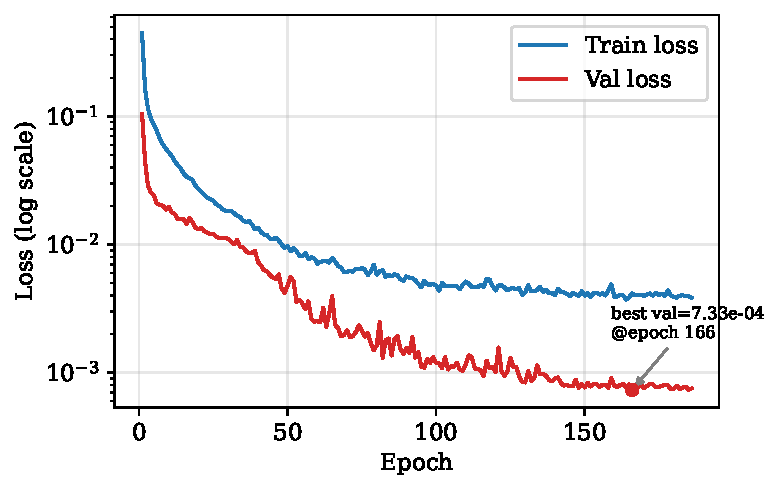
\includegraphics[width=0.92\linewidth]{figures/training_curve.pdf}
\caption{Neural network training. Validation loss tracks training loss with no over-fitting gap; the best model (epoch $166$, val loss $7.3\times10^{-4}$) is used for all reported results.}
\label{fig:train}
\end{figure}

\begin{figure}[t]
\centering
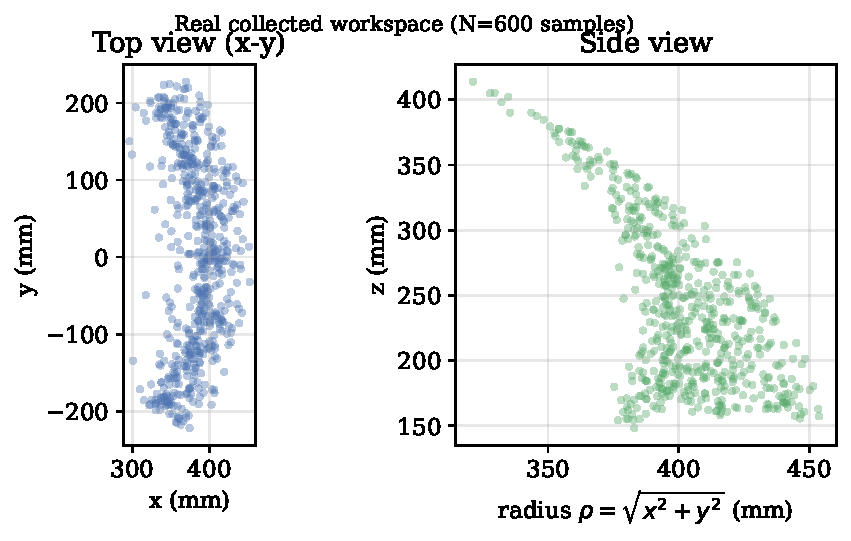
\includegraphics[width=0.99\linewidth]{figures/workspace.pdf}
\caption{Workspace covered by the $600$-configuration real dataset. The rejection sampler yields broad radial and vertical coverage while respecting the $z\ge192$~mm safety floor.}
\label{fig:workspace}
\end{figure}

\subsection{Software-Level Comparison}

Table~\ref{tab:software} reports the four methods on a common set of $50$ seeded, reachable targets, evaluated entirely in software (solution re-substituted into the same FK). To stress the solvers, each is given a deliberately \emph{far} initial guess (a random offset of $\sigma{=}0.3$~rad $\approx 17^{\circ}$ from the true configuration). The spread is enormous: more than two orders of magnitude between the best and worst method.

\begin{table}[t]
\centering
\caption{Software-level comparison ($N{=}50$, far initial guess).}
\label{tab:software}
\begin{tabular}{lccc}
\toprule
\textbf{Method} & \textbf{Mean err.\ (mm)} & \textbf{Success} & \textbf{Time (ms)} \\
\midrule
Analytical & $243.5$ & $4/50$ & $\mathbf{0.02}$ \\
Numerical (DLS) & $\mathbf{0.89}$ & $49/50$ & $32.8$ \\
Neural (MLP) & $17.2$ & $50/50$ & $0.80$ \\
Hybrid ($3$ steps) & $14.6$ & $50/50$ & $6.5$ \\
\bottomrule
\end{tabular}
\end{table}

Three points stand out. (1) The \emph{analytical} solver, exact in principle, is the \emph{worst} in practice: fed the nominal URDF link lengths, its closed-form assumptions are violated by the real geometry and it succeeds on only $4/50$ targets (mean $244$~mm). This is the parameter-sensitivity of closed-form IK made concrete, and the direct motivation for data-driven methods on this hardware. (2) The \emph{numerical} solver is the software accuracy champion at $0.9$~mm, but at $33$~ms per solve---slow, because a far initial guess forces many DLS iterations. (3) The \emph{neural} solver always returns a plausible in-limits solution in under $1$~ms, but its terminal precision ($17.2$~mm) is limited by the $600$-sample dataset. (4) The \emph{hybrid} solver, at a fixed budget of three DLS steps, improves only marginally over the raw network ($14.6$~mm): three steps are insufficient to recover from a far start. As the ablation in Section~\ref{sec:ablation} shows, the hybrid's accuracy is a smooth function of the step budget, reaching sub-millimeter \emph{median} error by $n{=}10$; the fixed-3-step configuration trades accuracy for a bounded $5$~ms latency.

\subsection{The Real-Robot Reality: A Common Mechanical Floor}
\label{sec:realfloor}

We then executed the numerical, neural, and hybrid solutions on the physical arm for a common set of targets and measured the achieved tool-tip pose. The result (Table~\ref{tab:real}, Fig.~\ref{fig:svr}) is the paper's central observation: \emph{the software ranking collapses}. A solver that was $17\times$ more accurate than another in software is statistically indistinguishable from it on hardware, because all methods land near a common $\sim\!34$~mm error.

\begin{table}[t]
\centering
\caption{Software vs.\ real-robot open-loop error (mm).}
\label{tab:real}
\begin{tabular}{lcc}
\toprule
\textbf{Method} & \textbf{Software err.} & \textbf{Real open-loop err.} \\
\midrule
Numerical (DLS) & $0.90$ & $35.6$ \\
Neural (MLP) & $15.2$ & $35.9$ \\
Hybrid ($3$ steps) & $5.1$ & $36.0$ \\
\bottomrule
\end{tabular}
\end{table}

\begin{figure}[t]
\centering
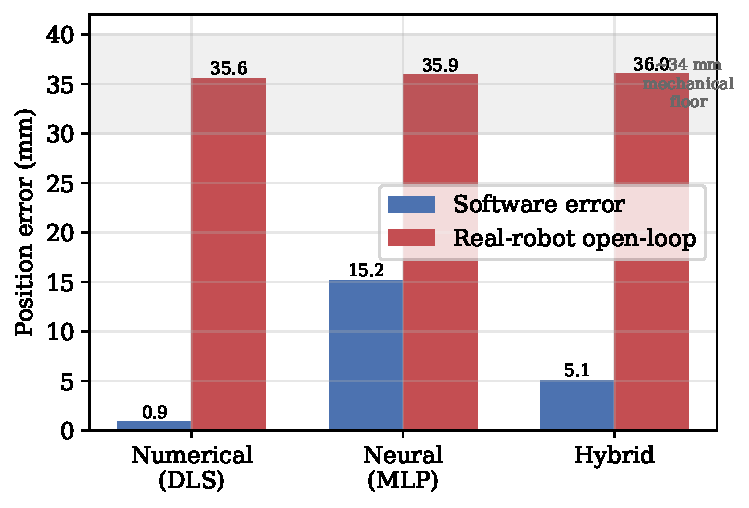
\includegraphics[width=0.92\linewidth]{figures/software_vs_real.pdf}
\caption{Software error (blue) varies by $17\times$ across methods, but real-robot open-loop error (red) is $\sim\!34$--$36$~mm for all of them: the mechanical floor (shaded) dominates.}
\label{fig:svr}
\end{figure}

\subsection{Error Decomposition: The Floor Is Mechanical}

Is the $34$~mm floor caused by residual IK error, or by the hardware? We isolate the two by \emph{removing IK entirely}: we command a set of joint angles directly, read the achieved angles back, and compare the FK tool position of commanded vs.\ achieved. This path contains no IK solver, so any error is purely mechanical (servo tracking, gravity sag, backlash, frame flex).

The directly-commanded configurations exhibit a $33.5$~mm mean tool displacement---essentially the entire floor. Decomposing per joint, the dominant term is a $\approx\!4.6^{\circ}$ droop of the shoulder-lift joint under the arm's own weight (the printed gears and low-cost servos yield under gravitational torque), which at the arm's $\sim\!0.4$~m reach maps to roughly $30$~mm of tip displacement. We conclude the floor is a \emph{mechanical} property of the arm, independent of the IK algorithm; this is precisely why the software ranking evaporates in Table~\ref{tab:real}.

\subsection{Breaking the Floor: Joint-Space Closed Loop}
\label{sec:closedloop}

If the error is a consistent mechanical offset, it should be correctable by feedback. Crucially, we have no external sensor (camera, motion-capture, or laser), so we cannot close the loop in \emph{task} space directly. But the servos report their own positions, so we can close the loop in \emph{joint} space: command $\mathbf{q}_{\mathrm{cmd}}$, read the achieved $\mathbf{q}_{\mathrm{act}}$, and correct toward the joint target the IK solver requested,
\begin{equation}
\mathbf{q}_{\mathrm{cmd}} \leftarrow \mathbf{q}_{\mathrm{cmd}} + 0.8\,(\mathbf{q}_{\mathrm{target}} - \mathbf{q}_{\mathrm{act}}),
\label{eq:cl}
\end{equation}
iterating until the joint residual is small. This drives the arm to actually \emph{hold} the joint angles the solver asked for, cancelling the servo-tracking and sag error at the joint level.

Over five test targets, this reduced the open-loop tool error from a mean of $33.6$~mm to $4.0$~mm---an $88\%$ reduction---in three to five iterations (Fig.~\ref{fig:cl}), using nothing but the built-in encoders. The residual $4$~mm reflects effects that are not observable at the joints (e.g., link flex and frame compliance downstream of the last encoder), which would require exteroceptive sensing to remove.

\begin{figure}[t]
\centering
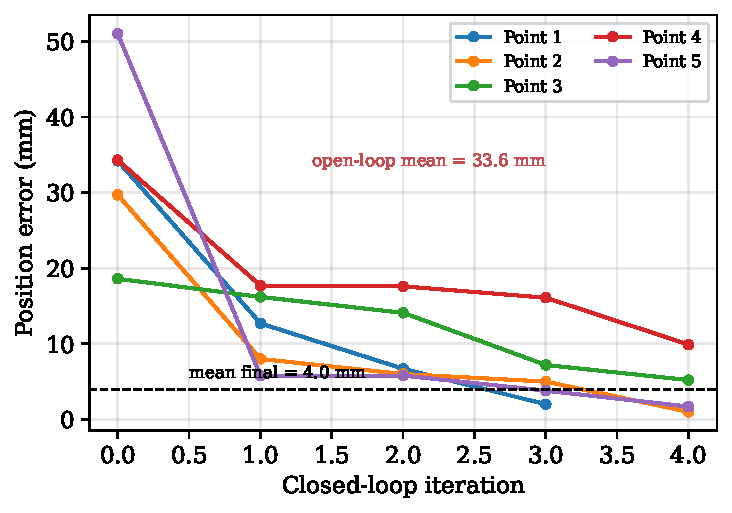
\includegraphics[width=0.92\linewidth]{figures/closed_loop.pdf}
\caption{Joint-space closed loop~\eqref{eq:cl}. All five targets converge from a $33.6$~mm open-loop mean to a $4.0$~mm mean within five iterations, using only proprioceptive encoder feedback.}
\label{fig:cl}
\end{figure}

\subsection{Ablation Studies}
\label{sec:ablation}

\textbf{Current-joint input.} Removing $\mathbf{q}^{\mathrm{cur}}$ from the input (7-D pose-only) forces the network to average over the elbow-up/down branches near configurations where both are feasible, injecting orientation error and joint discontinuities. Conditioning on the current state restores single-branch selection and is what makes a plain MLP viable for this multi-solution problem.

\textbf{Angle encoding.} Replacing the $(\sin\alpha,\cos\alpha,\sin\psi,\cos\psi)$ encoding with raw angles degrades convergence: samples straddling the $\pm180^{\circ}$ wrap are seen as distant despite being physically adjacent, and the network wastes capacity stitching the discontinuity.

\textbf{Hybrid refinement steps.} Figure~\ref{fig:ablation} sweeps the DLS step budget $n$ under the same far-initial-guess protocol. From the raw warm start ($n{=}0$, $17.2$~mm mean / $13.6$~mm median) the error is roughly flat through $n{=}3$ ($15.9$/$12.8$~mm), then falls steeply: $n{=}5$ gives $9.9$/$7.6$~mm and $n{=}10$ gives $5.7$~mm mean with a $0.9$~mm \emph{median}. The mean stays above the median throughout because a minority of far-start targets need still more iterations, but the median confirms the hybrid reaches numerical-grade precision on typical targets by $n{=}10$, at $11$~ms---still faster and more reliable than cold-started DLS from the same far guess. The knee of the curve is near $n{=}5$; the choice of $n$ is thus an explicit accuracy/latency dial rather than a fixed prescription.

\begin{figure}[t]
\centering
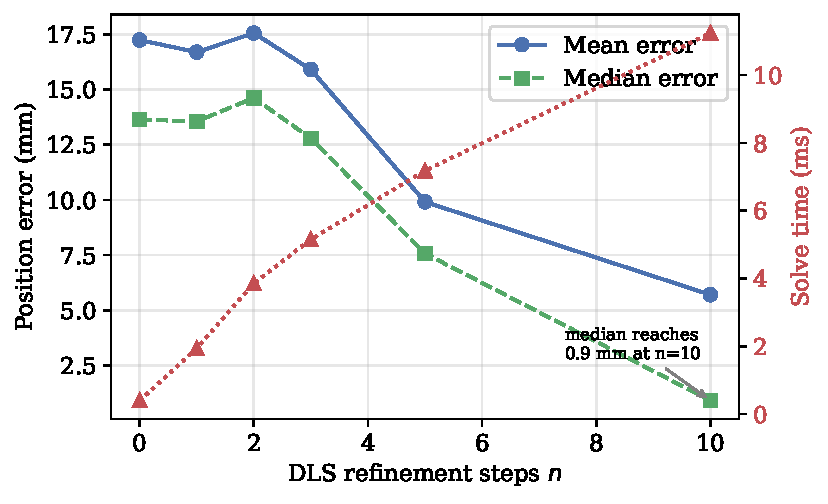
\includegraphics[width=0.92\linewidth]{figures/hybrid_ablation.pdf}
\caption{Hybrid IK ablation: position error (left axis) and solve time (right axis) vs.\ DLS refinement steps, from a far initial guess ($N{=}50$). Error is flat through $n{=}3$, then drops; the median reaches $0.9$~mm at $n{=}10$.}
\label{fig:ablation}
\end{figure}

\textbf{Tanh limit enforcement.} Across all evaluations the $\tanh$ output layer~\eqref{eq:tanh} produced zero joint-limit violations by construction, versus the post-hoc clipping that a linear output would require. The ablation is degenerate---the hard constraint cannot be violated---which is exactly its value.

\textbf{Dataset size and augmentation.} The $19$~mm software error of the pure network is dominated by the modest $600$-sample real dataset; the $K{=}10$ noise augmentation improves neighborhood robustness (recovery from a perturbed current state) but cannot manufacture pose coverage the real data lacks. This bounds how far a pure learned solver can go here and further motivates the hybrid design.

\subsection{Pitfalls and Lessons}
\label{sec:pitfalls}

Three engineering pitfalls materially affected results and are worth recording. (1) \emph{FK chain and tool offset:} an early FK bug (reversed joint order, gripper link included, missing base joint, missing $98$~mm handle) placed the modeled tip $\sim\!30$~cm off and drove the arm into the table; fixing the chain and adding the tool offset was a prerequisite for any valid measurement. (2) \emph{Task-space consistency:} the numerical solver only converges when the target pose is expressed in the \emph{same} task-space convention it uses internally; a mismatched Euler convention silently prevented convergence. (3) \emph{The shortcut trap} (Section~\ref{sec:neural}): a poorly constructed current-state distribution let the network copy its input, yielding a deceptively low validation loss and a $112$~mm hardware error. Each of these is invisible in a purely software metric and only surfaced on hardware---reinforcing the paper's theme that the real robot is the honest evaluator.

\section{Conclusion}

We compared analytical, numerical, neural, and hybrid IK on a low-cost 3D-printed SO-101 arm, in software and on hardware. In software the methods differ by more than two orders of magnitude; the numerical solver is the accuracy champion ($0.9$~mm) and the hybrid solver offers a tunable accuracy/latency trade-off that reaches numerical-grade median precision within about ten refinement steps while remaining robust to the far initial guesses that slow cold-started DLS. On the physical arm, however, all solvers collapse onto a common $\sim\!34$~mm error floor that we show, by a direct joint-command experiment, to be \emph{mechanical}---dominated by gravity-induced shoulder sag---and hence independent of the solver. Solver precision below this floor buys nothing in the real world.

The corollary is where the real leverage lies. A joint-space closed loop driven only by the servos' own encoders cut the real error by $88\%$ ($33.6\!\to\!4.0$~mm) with no external sensor. For low-cost manipulators, then, the engineering effort is better spent on feedback and calibration than on ever-more-precise open-loop solvers. The neural approach earns its place not by beating numerical precision but by tolerating the unknown parameters of a hand-built arm---the property that let it learn directly from real data where the analytical solver, fed nominal parameters, failed outright.

Future work: add an exteroceptive sensor (a single calibrated camera with a fiducial) to (i) close the loop in task space and remove the residual $4$~mm, and (ii) enable true real-robot \emph{training} on measured tool poses rather than FK-computed labels, eliminating the model-error term at its source. We also plan trajectory-tracking evaluation and a simplified single-length analytical model as a calibration baseline.

\section*{Reproducibility}
The four solvers, the FK model with tool offset, the safety-checked collection and closed-loop scripts, the $600$-sample real dataset, and the trained model are released with this paper.

\section*{Acknowledgment}
The authors thank the LeRobot community for open-source tools and hardware designs.

\begin{thebibliography}{00}
\bibitem{siciliano2016robotics} B. Siciliano and O. Khatib, Eds., \textit{Springer Handbook of Robotics}, 2nd ed. Springer, 2016.
\bibitem{craig2005introduction} J. J. Craig, \textit{Introduction to Robotics: Mechanics and Control}, 3rd ed. Pearson Prentice Hall, 2005.
\bibitem{buss2004introduction} S. R. Buss, ``Introduction to inverse kinematics with Jacobian transpose, pseudoinverse and damped least squares methods,'' \textit{IEEE Journal of Robotics and Automation}, vol.\ 17, pp.\ 1--19, 2004.
\bibitem{buss2005selectively} S. R. Buss and J.-S. Kim, ``Selectively damped least squares for inverse kinematics,'' \textit{Journal of Graphics Tools}, vol.\ 10, no.\ 3, pp.\ 37--49, 2005.
\bibitem{nakamura1986inverse} Y. Nakamura and H. Hanafusa, ``Inverse kinematic solutions with singularity robustness for robot manipulator control,'' \textit{ASME J.\ Dynamic Systems, Measurement, and Control}, vol.\ 108, no.\ 3, pp.\ 163--171, 1986.
\bibitem{wolovich1984simple} W. A. Wolovich and H. Elliott, ``A computational technique for inverse kinematics,'' in \textit{Proc.\ IEEE Conf.\ Decision and Control}, 1984, pp.\ 1359--1363.
\bibitem{paul1981robot} R. P. Paul, \textit{Robot Manipulators: Mathematics, Programming, and Control}. MIT Press, 1981.
\bibitem{duka2014neural} A.-V. Duka, ``Neural network based inverse kinematics solution for trajectory tracking of a robotic arm,'' \textit{Procedia Technology}, vol.\ 12, pp.\ 20--27, 2014.
\bibitem{bensadoun2022neural} R. Bensadoun, S. Gur, N. Blau, and L. Wolf, ``Neural inverse kinematics,'' in \textit{Proc.\ Int.\ Conf.\ Machine Learning (ICML)}, 2022, pp.\ 1787--1797.
\bibitem{malik2022deepnn} A. Malik, Y. Lischuk, T. Henderson, and R. Prazenica, ``A deep neural network approach for the solution of the inverse kinematics of a robotic manipulator,'' \textit{Robotics}, vol.\ 11, no.\ 2, art.\ 44, 2022.
\bibitem{limXGNN2025} A data-driven graph-neural warm-start for numerical IK refinement, \textit{Electronics (MDPI)}, vol.\ 15, no.\ 14, art.\ 3071, 2025.
\bibitem{volinski2023neuromorphic} A. Volinski, Y. Zaidel, A. Shalumov, T. DeWolf, L. Supic, and E. Ezra Tsur, ``Learning inverse kinematics using neural computational primitives on neuromorphic hardware,'' \textit{npj Robotics}, vol.\ 1, art.\ 1, 2023.
\end{thebibliography}

\end{document}
